%From the example above, we can see that in order to perform model checking on the closed-loop system, the heart model should not only cover all possible inputs to the pacemaker specified in the requirement, but also have enough details to resolve ambiguities of executions
%% that may introduce false-positives and false-negatives. 
%\figref{abs_tree} demonstrates a collection of heart conditions modeled by the EP heart models. 
%These models are definitely not exhaustive. 
%Model checking the pacemaker model with all these heart models will not guarantee absolute safety. 
%By using physiological abstraction rules (R1-R7 in \figref{abs_tree}), the heart conditions can be generalized and expand the possible inputs to the pacemaker. 
%The result is a heart model $H_{all}$ with only two node automata correspond to the inputs to the pacemaker. 
%By allowing both node automata to be able to send inputs to the pacemaker $[0,\infty]$msec after the last input, the heart model $H_{all}$ covers all possible inputs to the pacemaker. However, $H_{all}$ cannot distinguish the ELT condition from the healthy condition due to the lack of representation of ventricle to atrium conduction. 
%The heart model $H_{cond}$ models the conduction between the atrium and the ventricle with a path automata, thus is the appropriate heart model to evaluate ELT.
\section{Physiological Model Abstraction and Refinement}
%\todo[inline]{I would change the title. Multi-scale is not precise enough, and in hte context of biological modeling, might be understood as cellular to tissue to whole organ modeling - which isnt what this section describes. Perhaps use something more precise like "Modeling abstractions" or "Model Abstraction tree"}
From the example above, we can see that in order to perform model checking on the closed-loop system, the heart model should not only cover all possible inputs to the pacemaker specified in the requirements, but also have enough details to resolve ambiguities of executions that may introduce false-positives and/or false-negatives. 
 The left column of \figref{abs_tree} shows a collection of heart models each modeling a particular heart condition.  
However, these models do not cover \emph{all} possible heart conditions, thus model checking the pacemaker with each of these heart models will not guarantee absolute safety. 
%\figref{abs_tree} shows a collection of heart conditions modeled by the EP heart models. 
%These models do not cover all possible heart conditions, so model checking the pacemaker model with each of these heart models will not guarantee absolute safety. 
%\todo[inline]{The following sentence is ambiguous..."generalized", "expand", it's not clear what you mean. I suggest replacing it with ""}
Physiological abstraction rules (R1-R7 in \figref{abs_tree}) are defined to increase the behaviors of the original model(s), while guaranteeing new behaviors introduced can still be physiologically valid.
%By using physiological abstraction rules , the heart conditions can be generalized and expand the possible inputs to the pacemaker. 
As an example, abstraction rule R4 merges parameter ranges for heart models with the same node and path topologies.
Imagine two node automata $N1,N2$ can self-activate within [300,400]msec and [500,600]msec, respectively.
By applying R4, the new node automaton $N3$ can self-activate within [300,600]msec.
$N3$ covers all behaviors of $N1,N2$, plus new behaviors which are mostly physiologically valid.
If the physiologically-invalid behaviors introduced into $N3$ are returned by the model checker as evidence, they can be eliminated by refining $N3$ back to $N1,N2$.
%\todo[inline]{ZJ: I know it sounds sketchy, but how can we explain the whole idea of abstraction tree with several sentences?}
	%\todo[inline]{instead of a generic example, use actual parameter ranges for actual parameters. E.g. "For example, the rest period of one model being [300,320]ms, and for another model being [400,500]ms, rule R4 replaces these two models by a model whose rest period is the union [300,500]ms. }
%The new abstract model includes all behaviors of the merged heart models, plus new behaviors that may or may not be physiologically valid.}\todo[inline]{confusing, because we don't give a consequence of this. so what if they're not valid? how do we know if they're valid? Not valid sounds bad, is it? what point are we making? I suggest sticking to the example}.

By systematically applying the abstraction rules on the initial set of heart models, we get an abstraction tree  (\figref{abs_tree}) .
The root of the abstraction tree is a heart model $H_{all}$ with only two node automata corresponding to the inputs to the pacemaker.
By allowing both node automata to be able to send inputs to the pacemaker $[0,\infty]$msec after the last input, the heart model $H_{all}$ covers all possible inputs to the pacemaker. However, $H_{all}$ cannot distinguish the ELT condition from the healthy condition due to the lack of representation of ventricle to atrium conduction. 
The heart model $H_{cond}$ (\figref{abs_tree}) models the electrical conduction between the atria and the ventricles with a path automaton, thus is the appropriate heart model to evaluate ELT. 
Similarly, more complex properties will lead to appropriately detailed models along the Model Abstraction Tree.%\todo{first time you mention abstraction tree...}

\begin{figure}[t]
	\centering
	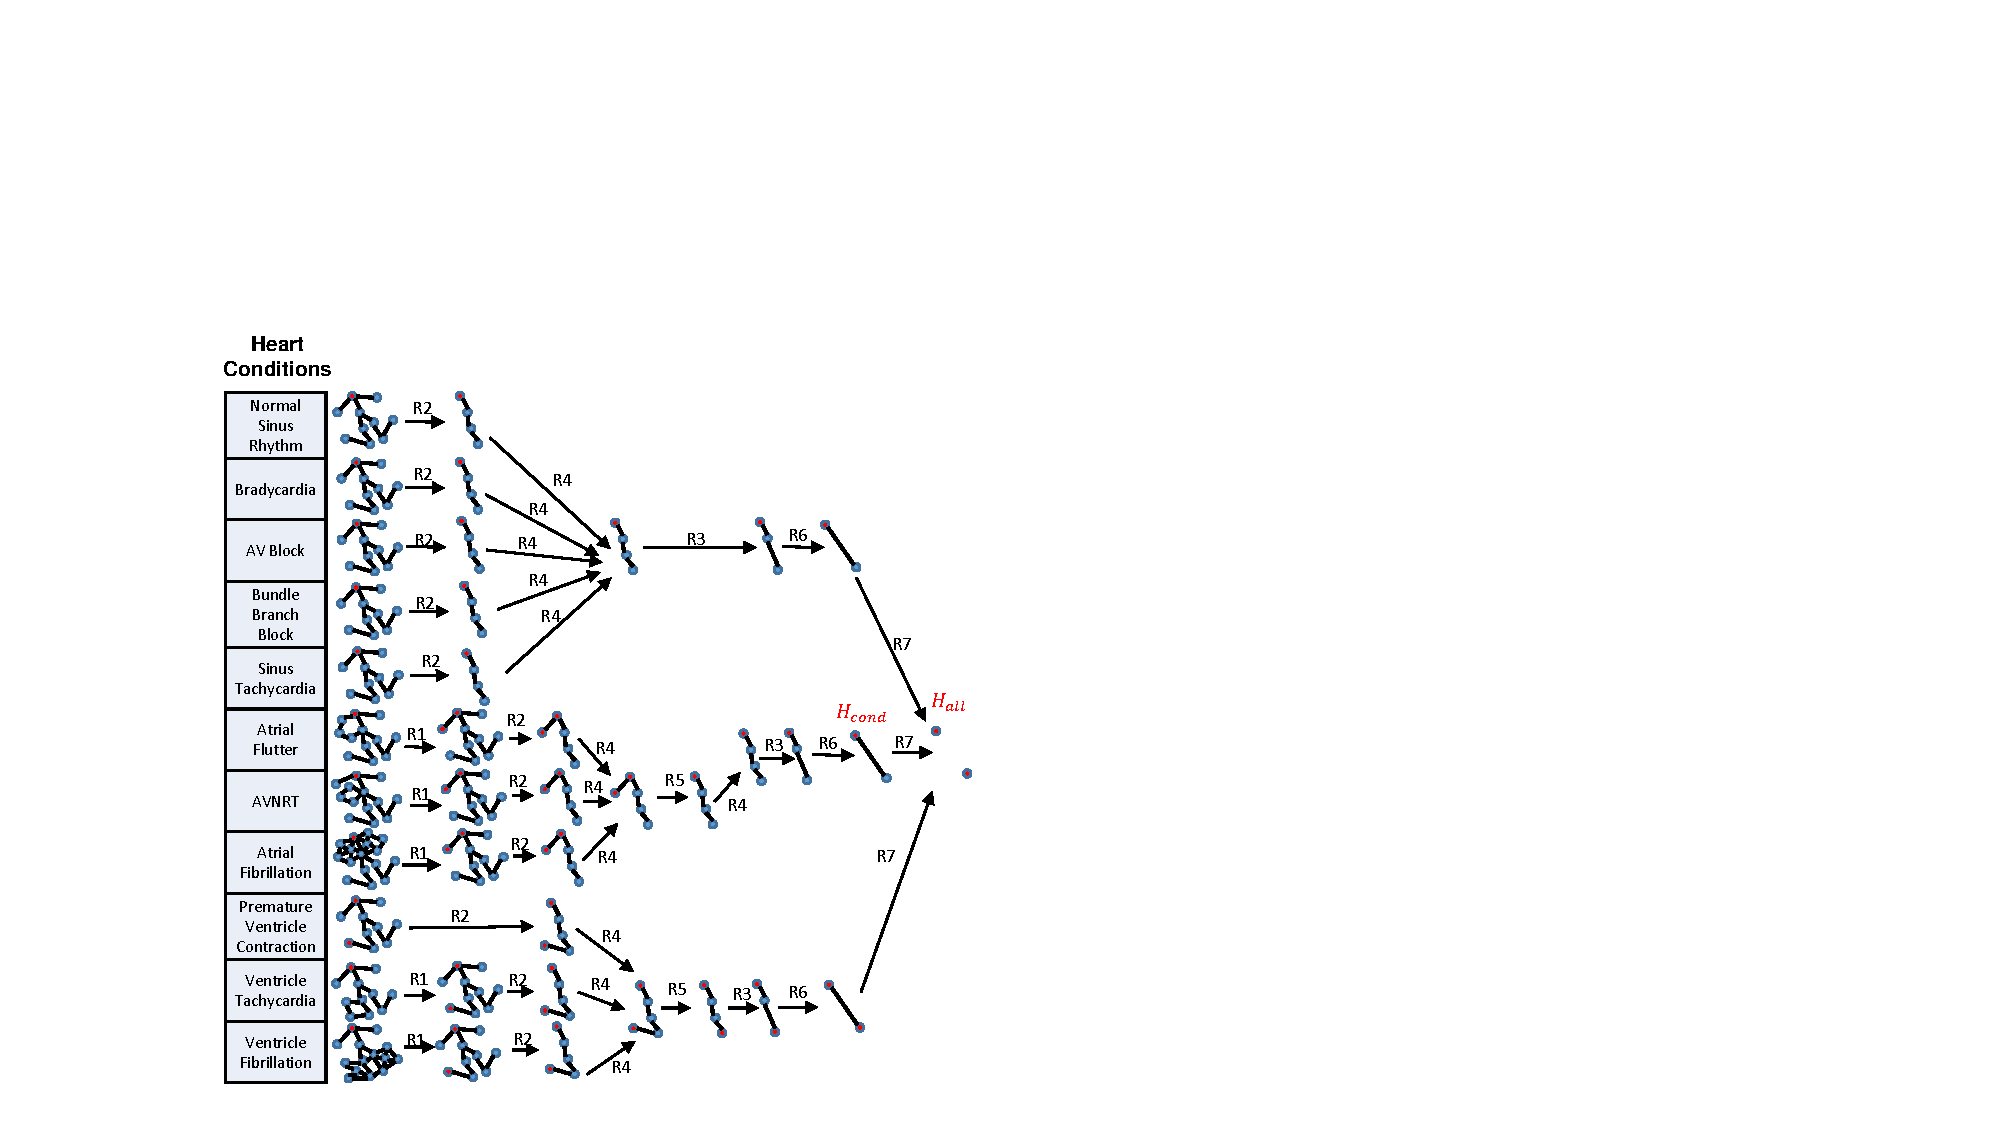
\includegraphics[width=\textwidth]{figs/abs_tree.pdf}
	\caption{\small Multi-scale modeling of the heart. The heart model at a higher level (further to the right) contains all possible inputs to the pacemaker from the heart models at previous levels}
	\label{fig:abs_tree}
\end{figure}